
\chapter{Mu2e Offline Event Reconstruction}\label{eventreco}

The primary goal of the Mu2e reconstruction algorithms is 
to efficiently reconstruct electrons within the specific range 
of conversion electrons. To meet this goal, the algorithms, 
along with certain user-defined parameters, are preconfigured 
with default values that are carefully optimized for this purpose. 
This appendix details the various stages involved in the Mu2e event reconstruction process.

\section{Hits reconstruction and pre-filtering}
\subsection{Tracker Hit Reconstruction and Pre-filtering}
Charged particles traversing the tracker volume generate 
ionization charges within the gas enclosed by the straws. 
These charges are collected and produce electrical signals. 
Since the straws are read out by the front-end electronics from 
both ends, the initial step in the hit reconstruction process 
involves combining the two resulting electrical signals to 
estimate both the hit time and position along the wire. In the 
reconstruction code, this information is encapsulated in an object named $StrawHit$.

One of the most significant challenges in track reconstruction within 
the Mu2e experiment is the presence of numerous $StrawHit$ 
objects within the 1.7$\mu$s time window that corresponds to 
a single event. The first critical task is, therefore, to identify 
$StrawHit$ instances that are close in time and likely to 
have been generated by the same particle traversing the tracker. To 
enhance spatial resolution and minimize combinatorial complexities 
during track searching, adjacent $StrawHit$ objects within a 
panel, which are most likely due to the same particle, are combined 
into a more complex object termed $ComboHit$. While retaining 
the information from individual $StrawHit$s, the $ComboHit$ provides the average time and position of the cluster.

This process is complicated by the presence of numerous hits produced 
by low-energy $p < 20$ MeV/c electrons, which are knocked 
out by Compton scattering, $\gamma$ conversion, or $\delta$-rays. 
These electrons, commonly referred to as $\delta$-electrons, follow 
trajectories with small radii and can generate a large number of hits, 
all confined within a limited volume, leading to regions of high occupancy. 
Fortunately, the hit patterns generated by $\delta$-electrons are markedly 
different from those generated by particles within the energy range of 
interest for Mu2e, as further discussed in Chapter \ref{delta}. These can be 
identified and filtered out using either the $FlagBkgHits$ or $DeltaFinder$ algorithms.

At this stage of the reconstruction process, the tracker's information 
has been translated into a collection of $ComboHit$ objects. 
Each $ComboHit$ is the result of combining a set of associated 
$StrawHit$s and is characterized by its specific time and position. 
The clustering algorithm employed not only aids in this combination but also 
facilitates a partial reduction and filtering of background hits due to secondary electrons.


\subsection{Calorimeter Hit Reconstruction}
The logical equivalent of a $ComboHit$ in the tracker is termed a $Cluster$ in 
the calorimeter. A $Cluster$ is formed by combining the signals generated by a 
group of crystals when a particle impacts the detector. The reconstruction of a 
$Cluster$ begins by identifying the crystal with the highest energy deposition 
and subsequently adding all adjacent crystals that produce signals within a 
2 ns window and have an energy above 50 MeV.

$Cluster$s are constructed by aggregating signals from crystals struck by 
particles in the calorimeter. The reconstruction process involves grouping 
adjacent crystals within a 2 ns time window, with an adjustable energy 
threshold, currently set at 50 MeV. This procedure is iteratively applied, 
starting from the added crystals, until no further crystals meet the inclusion 
criteria. Given the precision of the time measurements provided by the 
calorimeter, the timing of a $Cluster$ can be utilized to define a temporal 
window within which all $ComboHit$s generated by a particle passing through 
the tracker should be located. Thus, the calorimeter plays a crucial role in 
seeding the pattern recognition process, significantly reducing the 
combinatorial background in the tracker.


\section{Helix Search}
The primary objective of the Mu2e tracking software 
is to reconstruct the trajectories of charged particles 
moving within the magnetic field of the Detector Solenoid. 
Ideally, these trajectories would form helices if no other effects were involved.

The helical paths can be described by the following set of parameters:

\[
\vec{\eta} \equiv (d_0, \phi_0, \omega, z_0, \tan \lambda)
\]

where $d_0$ represents the distance of the point of closest 
approach to the solenoid axis in the $x-y$ plane, with its 
sign determined by the particle's angular momentum relative 
to the origin. $\phi_0$ denotes the direction of the momentum 
at the point of closest approach, while $\omega = 1/R$ is the 
curvature in the transverse plane. $z_0$ is the $z$-coordinate 
at the point of closest approach, and $90^\circ - \lambda$ 
defines the pitch angle between the momentum vector $\vec{p}$ and the $xy$ plane.

The number of full rotations completed by a particle within 
the tracker volume is a function of its pitch and momentum. 
Most particles of interest in the Mu2e experiment complete 
more than one full rotation, implying that the actual trajectory 
for most tracks will be a long helix rather than just a segment 
of one. Due to the detector's design, particles may develop a 
portion of their trajectories within the bore, resulting in 
sequences of hits in the tracker that form multiple arcs.

The combination of $ComboHit$s in the tracker, alongside the 
potential simultaneous presence of $Cluster$s in the calorimeter, 
forms the foundational data required to reconstruct the helical 
trajectories. This search is executed in two successive phases, 
known respectively as $TimeClustering$ and $Pattern-Recognition$.
\subsection{Time Clustering}
Given that the duration of a Mu2e event is several orders of 
magnitude longer than the time it takes for a particle to 
traverse the tracker, the first essential task is to identify 
which $ComboHit$s could have originated from the same particle. 
This can be achieved by analyzing the time distribution of the $ComboHit$s.

The procedure can be logically divided into two main steps:

\begin{itemize}
\item \textbf{Analyzing the $ComboHit$s Time Distribution}: 
$ComboHit$s produced by the same particle typically cluster 
into peaks within the time distribution. At each peak, a new 
entity known as a $TimeCluster$ is created, and the collection 
of $ComboHit$s associated with that peak is assigned to this 
$TimeCluster$. To enhance the accuracy of associating $ComboHit$s 
with $TimeCluster$s, the time distribution is adjusted by 
propagating all hit times to the central plane of the tracker 
($z = 0$). This propagation is performed by assuming values for 
$\beta$ and the angular velocity $\lambda$, which depend on the 
hypothesized particle identity. Similar to how $ComboHit$s are 
formed from $StrawHit$s, the $TimeCluster$ consists of a list of 
$ComboHit$s, but it is also associated with a time and position, 
both estimated from the $ComboHit$s;
\item \textbf{Refining the $ComboHit$s Collection}: The time and 
position of the $TimeCluster$ are subsequently used to further 
refine the collection of associated $ComboHit$s. Several criteria 
are applied to the $ComboHit$s linked with each $TimeCluster$, 
such as a maximum angular distance in the transverse $x-y$ plane. 
Following this refinement, the list of $ComboHit$s associated with 
the $TimeCluster$ may undergo minor adjustments. At this stage, 
the time and position of the $TimeCluster$ are re-evaluated, and 
an additional iteration may include $ComboHit$s that now meet 
the selection criteria. This iterative process continues until 
the list of $ComboHit$s associated with the $TimeCluster$ 
stabilizes, meaning no more $ComboHit$s are added or removed.

\end{itemize}
It is important to consider that the avalanche processes 
occurring within the straws have a finite velocity, and 
these avalanches are initiated at random distances from 
the wires. Given that the radius of a straw is 2.5 mm, 
the standard deviation of the uniform distribution for 
the distance between the avalanche's starting point and 
the wire can be approximately estimated through a 
back-of-the-envelope calculation as 2.5 mm/$\sqrt{12} \sim 700,\mu\text{m}$. 
Assuming a drift velocity of 50 $\mu\text{m}/\text{ns}$, this leads 
to a width estimate of approximately 14 ns. On the other hand, the 
hit times are propagated based on an assumed particle identity 
(specified by $\beta$ and pitch), meaning that $TimeCluster$s 
generated by different particles (with varying $\beta$) will 
have small differences and a similar spread in time.

The entire procedure is slightly modified if an energy cluster 
is detected in the calorimeter. In this case, the cluster can 
define the time window and provide a rough estimate of the 
$TimeCluster$'s $x-y$ position. Once this procedure is complete, 
all $TimeCluster$s containing more than a programmable number of hits are stored.
\subsection{Pattern Recognition}
The next step involves searching for patterns 
within the list of $TimeCluster$s. The current Mu2e 
code implements two primary pattern recognition algorithms. 
Pattern recognition in Mu2e is categorized into two main 
approaches: Tracker-only Pattern Recognition and Calorimeter + Tracker Pattern Recognition.

\subsubsection{TrkPatRec: Tracker-only Pattern Recognition}

The Tracker-only Pattern Recognition algorithm, referred 
to as $TrkPatRec$ in Mu2e terminology, follows a two-step 
process. Initially, $TrkPatRec$ analyzes the $x$-$y$ plane 
to find the track projection on the transverse plane. This 
analysis determines the track's radius (which is correlated 
with the transverse momentum) and the impact parameter with 
respect to the Stopping Target. Subsequently, the 
reconstruction in the $\phi$-$z$ plane is carried out, 
where the $2\pi$ ambiguity is resolved, and the track pitch is determined.

\paragraph{Reconstruction in the $x$-$y$ plane}

To identify the optimal circle that fits the hit distribution, 
a loop is executed over all possible triplets of 
$ComboHit$s that belong to the same $TimeCluster$. 
For each triplet, if it spans a sufficient area, the 
$(x, y)$ coordinates of the intersection of the two 
perpendicular bisectors are recorded. The median operator 
is then employed to combine the results from all triplets, 
yielding a point that represents a stable approximation of 
the helix center. Once the circle's center is established, 
a second loop determines the radial distance of the 
$ComboHit$s from the helix axis, providing information 
about the track's radius. A pictorial representation of 
this procedure is shown in Figure \ref{fig:trkpatrec}.
\begin{figure}[!h]
    \centering
    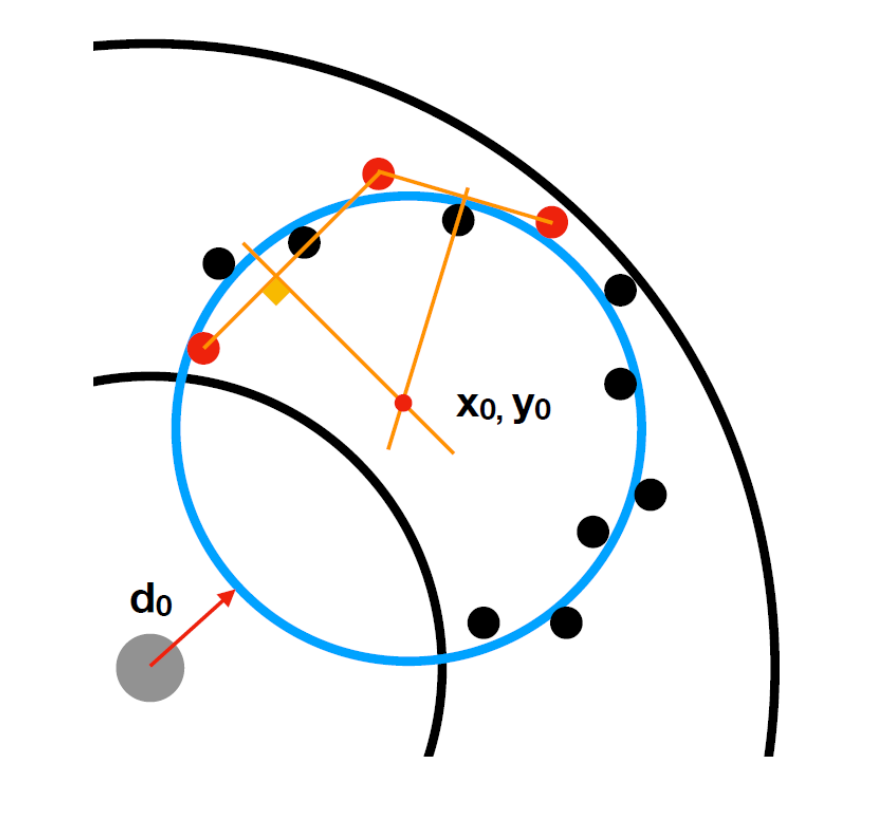
\includegraphics[width =0.4\textwidth]{figures/png/Screenshot_20240810_160341.png}
    \caption[Procedure adopted to search for the center of the $x-y$
    projection of the helix.]{A pictorial representation of the procedure 
    used to search for the center of the helix's $x$-$y$ projection using 
    triplets of $ComboHits$ is shown. If a triplet covers a sufficient area, 
    the position of the intersection of the 
    bisectors is recorded. The median of these points provides an 
    estimate of the helix axis \cite{trkpat}.}
    \label{fig:trkpatrec}
\end{figure}
\paragraph{Reconstruction on $\phi-z$ plane}
To estimate the pitch of the track, the first step 
is to resolve the $2\pi$ ambiguity associated with the 
angular position of the hits. Specifically, the angular 
positions $\phi$ of hits generated in the $n$-th loop of 
the track must be shifted by $2\pi n$. To make this 
correction, the angular velocity $\frac{d\phi}{dz} = \frac{1}{\lambda}$ 
of the particle is required, and therefore the first necessary 
step is to estimate $\frac{1}{\lambda}$.

A histogram is created using the variable $\lambda_{i,j;k}$, defined as:
\begin{equation}
    \frac{1}{\lambda_{i, j ; k}}=\frac{\left(\phi_j+2 \pi k\right)-\phi_i}{z_j-z_i}
\end{equation}
where $i$ and $j$ denote two different hits and range 
from $0$ to $NCH -1$, while $k$ accounts for the number 
of full rotations, ranging from $0$ to $10$. The peaks in 
the resulting distribution are used to assign hits to the 
corresponding $k$-th loop, thereby resolving the ambiguity.

Figure \ref{fig:ambiguity} illustrates how resolving the 
ambiguity affects the position of the hits in the $\phi - z$ plane. 
Once the ambiguity is resolved, it is possible to generate the 
histogram for $\frac{1}{\lambda_{i,j}} = \frac{\phi_j - \phi_i}{z_j - z_i}$, 
where the peak provides the best estimate of the helix's $\frac{d\phi}{dz}$.

\begin{figure}[!h]
    \centering
    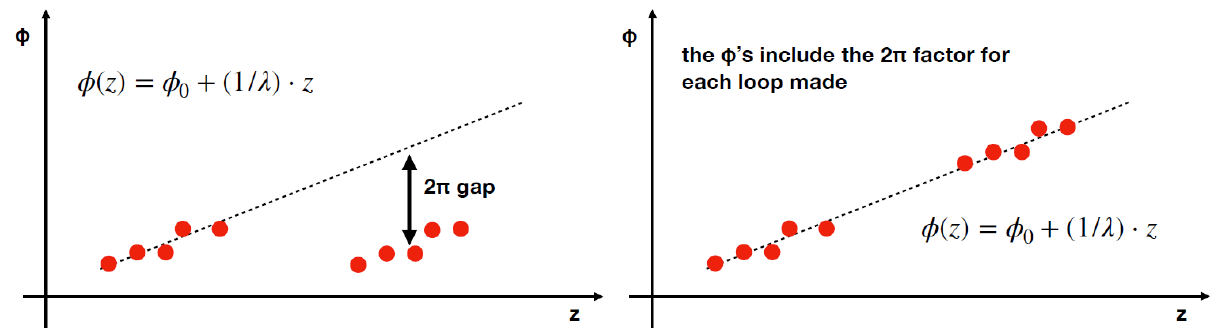
\includegraphics[width =\textwidth]{figures/png/Screenshot_20240810_160405.png}
    \caption[Sketch of the resolution of the 2$\pi$ ambiguity.]{Sketch illustrating the resolution of the 2$\pi$ ambiguity. 
    Assigning the hits to the correct loop enables the determination of the track's angular velocity.}
    \label{fig:ambiguity}
\end{figure}

\subsubsection{CalPatRec: Calorimeter+Tracker Pattern Recognition}

The $CalPatRec$ algorithm utilizes $CaloCluster$s as initial $seeds$ for 
pattern recognition. If a $CaloCluster$ with reconstructed energy exceeding 
50 MeV is present, its time and position are used to filter the $ComboHit$ 
collection. The selected hits must fall within a $\pm 40$ ns window relative 
to the calorimeter cluster's time and must lie within the same semi-plane 
(Figure \ref{fig:combinatorial}). This region is defined by first 
determining the angular position of the $Cluster$ with respect to the 
beam axis. The tracker is then divided into two halves using a plane 
perpendicular to the $Cluster$'s position vector that passes through 
the beam axis. The half that contains the $Cluster$ is retained.

Instead of using triplets of hits, the $CalPatRec$ algorithm begins with 
the calorimeter cluster position, one $ComboHit$, and the solenoid 
center as initial points. A loop over the $ComboHit$s allows the 
algorithm to flag hits that are sufficiently close to the helix projection. 
At this stage, the solenoid center can be dropped as a fixed position, and 
different $ComboHit$s are iteratively used to adjust the helix parameters. 
The parameters are updated using two separate reduced-$\chi^2$ fits for the 
$x$-$y$ and $\phi$-$z$ planes. A critical step in this process is the 
accurate projection of hit uncertainties, accounting for the orientation 
of the straws relative to the helix.


\begin{figure}[!h]
    \centering
    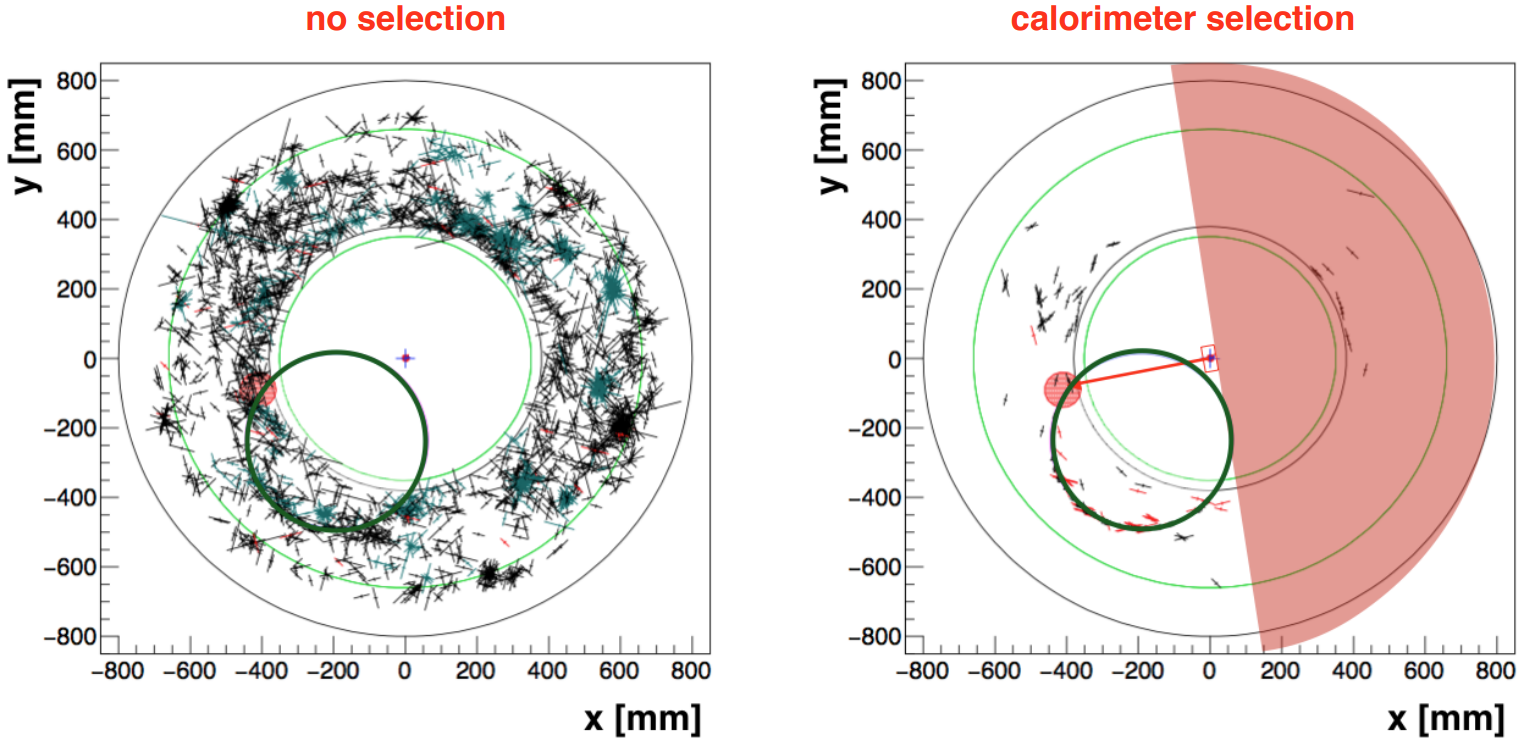
\includegraphics[width =0.8\textwidth]{figures/png/Screenshot_20240810_165014.png}
    \caption[Combinatorial background reduction achieved by exploiting the calorime-
    ter clusters seeding.]{Combinatorial background reduction achieved by exploiting the calorime-
    ter clusters seeding \cite{trkpat}. (Left plot) Typical Mu2e event 
    with a conversion electron
    projected on the $x-y$ plane. The green circle represents 
    the transverse projection of the
    conversion electron trajectory and the black crosses are $StrawHit$s (the long arm 
    indicates the direction of the straw); (Right plot) Same event 
    after applying the calorimeter seeding.}
    \label{fig:combinatorial}
\end{figure}


\section{Kalman Fitting}
After the pattern recognition algorithms have been executed, 
an initial estimate of the track parameters $\vec{\eta}$ becomes 
available. At this stage, there are still numerous effects that 
must be accounted for to optimize track reconstruction. Some of 
these effects are straightforward, such as the non-uniformity of 
the magnetic field, while others are subtler. For instance, there 
is an intrinsic symmetry in a straw hit regarding which side the 
particle traversed, leading to what is commonly referred to as 
ambiguity, as illustrated in Figure \ref{fig:trackam}.

\begin{figure}[!h]
    \centering
    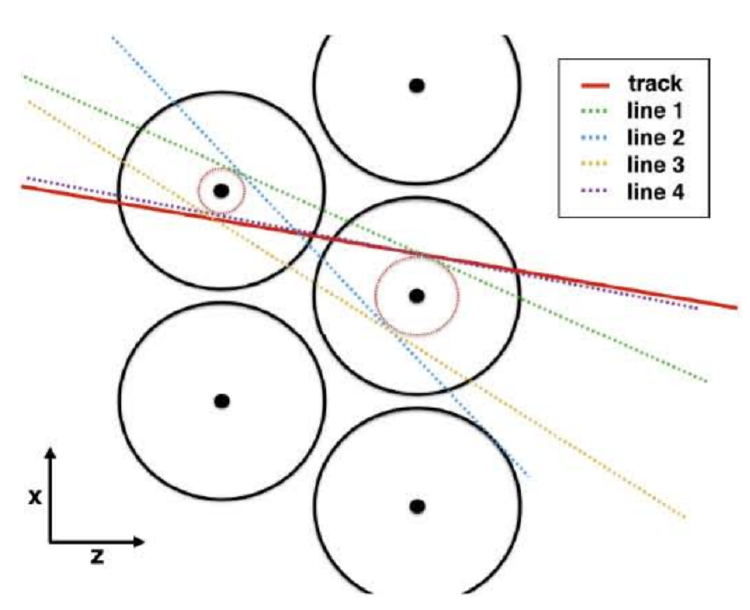
\includegraphics[width =0.8\textwidth]{figures/png/Screenshot_20240810_171118.png}
    \caption[The symmetry of the straw generates an ambiguity for the hits.]{The 
    symmetry of the straw generates an ambiguity for the hits.}
    \label{fig:trackam}
\end{figure}
To address these effects that influence particle trajectories, 
the well-established Kalman fitting algorithm is employed. The 
Mu2e experiment utilizes a fitter developed for the BaBar experiment. 
The standard fitting process begins with a simplified Kalman fit, 
known as KSF in the Mu2e offline framework. Although this initial 
fit does not account for all effects, such as particle interactions 
with detector material, it improves the accuracy of track parameter reconstruction.

For more comprehensive effect corrections, a second Kalman fit 
(referred to as KK in Mu2e Offline) can be applied to account 
for residual effects. In this approach, the parameter vector 
$\vec{\eta}$ and the position along the beam axis ($z$) are used 
for track optimization, denoted as $F(\vec{\eta}; z)$. This fitting 
process provides the optimal estimate of $\vec{\eta}$, along with 
the corresponding $5 \times 5$ covariance matrix $V$. The 
complexity of this process increases when the parameter vector 
depends on the running variable, $\vec{\eta}(z)$, which is the 
case in the Mu2e experiment.

In the momentum range of interest, around $p \sim 100$ MeV/c, 
different charged particle species, including electrons, muons, 
and protons, exhibit distinct behaviors within the Mu2e tracker. 
Electrons are highly relativistic with $\beta_e = v_e/c \sim 1$, 
while muons are significantly slower with $\beta_\mu \sim 0.7$. 
Protons at 100 MeV/c are deeply non-relativistic. The energy loss 
characteristics also differ among these particles. Electrons and 
muons experience energy losses on the order of 1-2 MeV in the tracker, 
which is small compared to their total energy. Conversely, protons 
primarily lose all their energy due to ionization in the tracker. 
To account for these diverse cases, the offline track reconstruction 
involves multiple passes, each assuming specific hypotheses about 
particle mass and propagation direction.



